\pagestyle{fancy}

\graphicspath{ {Figures/Chapter2_BeamMatterInteraction/} }

While in-depth dissertations about the broad topic of particles interaction with matter can be found in literature~\parencite*[]{ref:Knoll,ref:Evans,ref:avernier}, 
this chapter will introduce the basics  necessary to introduce the subject and understand later chapters.

The interactions that we will focus on are primarily those related to Coulomb forces between the incident charged particle and the electrons and nuclei of the detector material. During these interactions, the incident charged particle loses its energy and can be deflected from its original path. In the case of heavy charged particles whose rest mass is large compared with that of the atomic electron, inelastic collisions with atomic electrons are usually the predominant interaction mechanism. In such encounters, the electrons in the medium might experience a transition to an excited state (excitation) or to an unbound state (ionization). 

\subsection{The Bethe Bloch Formula}
\label{sec:Bethe}

Stopping power is the parameter used to describe the gradual loss of energy of a charged particle as it penetrates into a medium. For a given incident heavy particle and target, this energy loss is highly dependent on the particle velocity. At moderately relativistic energy ranges ($10$ - $10^6$ \si[]{\mega \electronvolt}/amu), the electrostatic stopping power is well defined by the Bethe Bloch theory \parencite[]{ref:Bethe}. 

\begin{equation}
    - \left< \frac{dE}{dx} \right> = Kz^2_e\frac{Z}{A}\frac{1}{\beta^2}\left[ \frac{1}{2} ln \left( \frac{2m_e c^2 \beta^2 \gamma^2 T_{max}}{I^2}\right) -\beta^2 - \frac{\delta\left(\beta \gamma\right)}{2} \right]
    \label{eq:bethe}
\end{equation}

With the symbol and parameter definitions given in table \ref{tab:ParBethe}. The mean ionization energy is highly dependent on the material, and it can vary from a few \si[]{\electronvolt} for materials with low Z to a hundred of \si[]{\electronvolt} for materials with high Z. A good approximation can be formulated as follows \parencite*[][]{ref:IonizationEne}:

\begin{equation}
    I \left[ eV \right] = 10 \cdot Z 
    \label{eq:ionizationEnergy}
\end{equation}

The maximum energy that can be transferred to a target electron in a single head-on collision is described by $T_{max}$, and can be approximated by the following formula \parencite*[][]{ref:TmaxFormula}: 
\begin{equation}
    T_{max} = \frac{2m_e c^2 \beta^2 \gamma^2}{1+\frac{\gamma m_e c^2}{M c^2}+\left( \frac{m_e c^2}{M c^2} \right)^2}
    \label{eq:tmax}
\end{equation}

Finally, $\delta (\beta \gamma)$ is a parametrized density correction factor necessary for highly relativistic particles \parencite*[][]{ref:Bethe}, its units are $MeV cm^2 g^{-1}$. It is important to notice that the energy deposited will very much depend on the characteristics of the incident particle as well as the absorber $\left( -\left< \frac{dE}{dx} \right> \propto \frac{Z}{A}  \right)$. 

\begin{table}[h!]
    \centering
    \begin{tabular}{ccc}
    \hline
    \textbf{Symbol}                  & \textbf{Definition}                  & \textbf{Units or Value}                                               \\ \hline
    $N_A$                      & Avogadro's Number           & $6.0221415(10)\cdot10^23$ $mol^{-1}$ \\
    $z_e$                      & Charge of incident particle &                                                              \\
    Z                       & Atomic number of absorber   &                                                              \\
    A                       & Mass Number of absorber     &                                                              \\
    I                       & Mean excitation energy      & eV                                                           \\
    $\beta \gamma$              & Relativistic parameters     &                                                              \\
    $m_e c^2$ & Electron Mass $\cdot$ $c^2$          & 0.510998918(44) MeV                                          \\
    $r_e$                      & Clasical Electron Radius    & 2.8179403250(28) fm                                          \\
    M                       & Incident Particle Mass      & $MeV/c^2$\\
    
    K/A                     & $4 \pi N_A r_e^2 m_e c^2/A$ & 0.307075 $MeV g^{-1} cm^2$  \\
     $\alpha$ & fine-structure constant & 1/137 \\ 
     \hline
    \end{tabular}
    \caption{Summary of variables used in this section.}
    \label{tab:ParBethe}
\end{table}

 Figure \ref{fig:EneDep} shows as an example, a comparison between the energy deposition of protons for different materials, as a function of the incident particle energy.  In this particular case, when the material is assumed to be thin, the energy deposition increases until reaching a maximum, after which it starts decreasing. From the image, we can observe that the energy deposited in graphite and copper is larger, due to their smaller mass number. Tungsten, gold and lead present smaller energy deposition values, and are similar to one another, due to their close atomic mass number. 

 \begin{figure}[h]
    \centering
    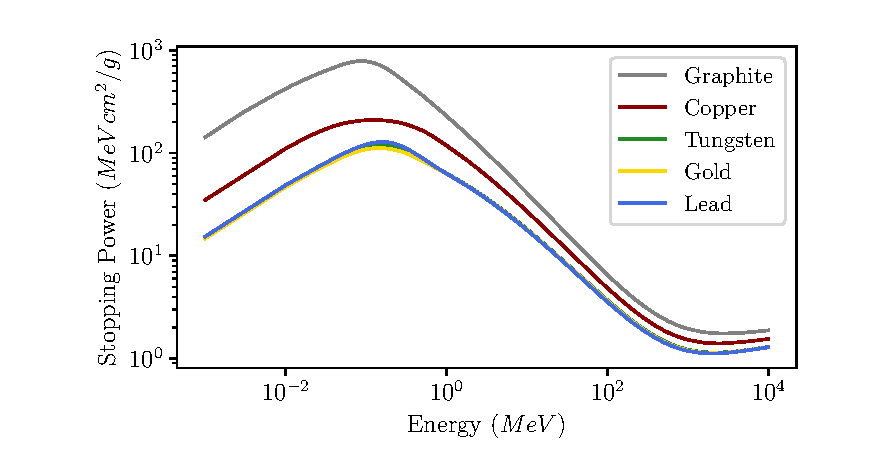
\includegraphics[width=1.0\columnwidth]{EdepMetal/EneDepMetal.pdf}
    \caption{Stopping power of protons in thin foils of different materials, as a function of incident particle energy. From \parencite*[][]{ref:NIST}.}
    \label{fig:EneDep}
\end{figure}

\subsection{Energy Loss in Mixtures and Compounds.}

One can consider a compound to be made up of very thin layers of pure elements in the right proportion. That is: 

 \begin{equation}
    \frac{dE}{dx} =  \sum w_j \left.\frac{dE}{dx} \right\vert_j
 \end{equation}

Where $\left. \frac{dE}{dx}\right\vert_j$  is the energy loss in the j-th component. However, it is important to remember that this is an approximation. The values of I and $\delta (\beta\gamma)$ are not perfectly represented by this addition method. More accurate values can be found in \parencite*[][]{ref:compound1} and \parencite*[][]{ref:compound2}, which include measured coefficients for nearly 200 mixtures and compounds. 

\subsection{Electrons Energy Loss}

For light particles such as electrons, bremsstrahlung losses are not negligible and can become dominant for energies above a few tens of \si[]{\mega\electronvolt}. One can define the critical energy $(E_c)$ as the point where the loss rates by Ionization and bremsstrahlung are the same \parencite*[][]{ref:EleCricEne}. 
\begin{equation}
    E_c = \frac{800}{Z + 1.2}
    \label{eq:ec}
\end{equation}

Figure \ref{fig:BremssVSion} shows the stopping power of electrons in a thin tungsten target, where we can observe the contribution of the radiative and collision interactions to the energy loss. In this case, radiative losses become relevant for incident electron energies $> 10 $\si[]{\mega\electronvolt}. This quantity is in agreement with equation \ref{eq:ec}.  

Some more information about how to model the energy losses due to this process can be found in \parencite*[][]{ref:BremstutorialG4}. However, in this thesis bremsstrahlung losses will be neglected, as we will always remain under the critical energy. 

\begin{figure}[h]
    \centering
    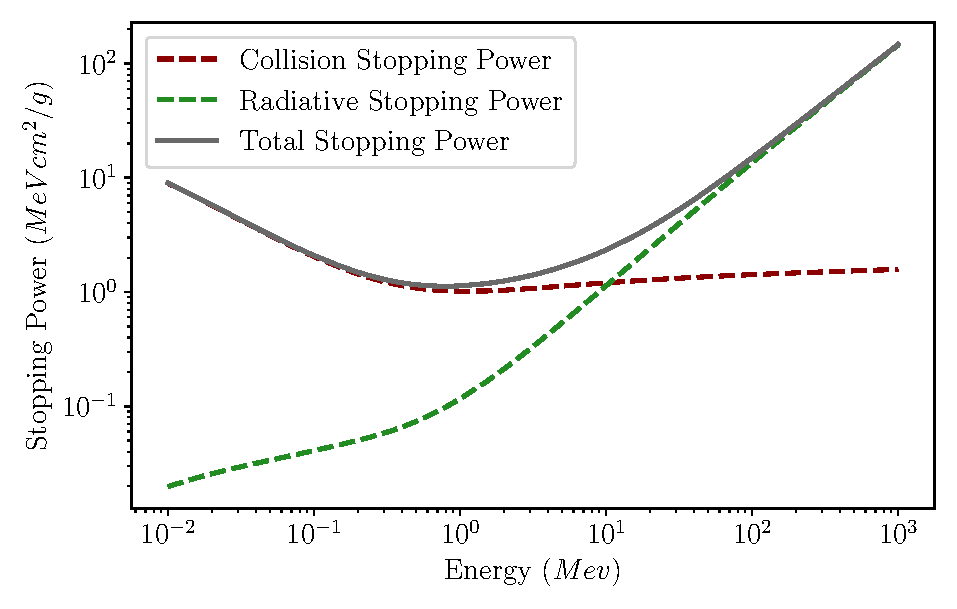
\includegraphics[width=1.0\columnwidth]{Electron_Edep/ElectronEdep.pdf}
    \caption{Stopping power of electrons in a thing tungsten foil, as a function of incident particle energy. From \parencite*[][]{ref:NIST}}
    \label{fig:BremssVSion}
\end{figure}

\subsection{Multiple scattering and Backscattering}
\label{sus:Scatt}

While traversing the material, the particle can be deflected from its original path. Most of these deflections occur due to Coulomb scattering with the atomic nucleus (Rutherford-type collisions). These collisions result in small angular deflections ( if $m_{nucleus} >> m_{particle}$ ). Figure \ref{fig:PartScattering} (left) shows a schematic representation of this process. 

The thicker the absorber and the larger its atomic number Z, the greater the likelihood that the incident particle will suffer multiple scatting events. Generally, 20 collisions are deemed sufficient to consider multiple scattering. Multiple scattering can be treated statistically if the number of successive encounters is high enough. This is well represented by the theory of Moliere \parencite*[][]{ref:Moliere}, which assumes that after a distance L traveled through the material, the angular distribution of the particles with respect to their initial direction is Gaussian in shape and centered around the direction of the incident particles. This assumes that the deflection angle is very small ($\theta \leq 10 \deg $). In these conditions, the mean square angle of such a Gaussian distribution can be calculated as follows: 

\begin{equation}
    \theta_0 = \frac{13.6 MeV}{\beta p c} z \sqrt{\frac{l}{X_0}}\left[ 1+0.038ln\left(\frac{l}{X_0}\right)\right] 
    \label{eq:multscat}
\end{equation}

$l/X_0$ is the thickness of the medium, described in terms of the radiation length ($X_0$), discussed in the next section. p, $\beta$ and z are the momentum, velocity and charge number of the incident particle. Experimental measurements show excellent agreement with the Gaussian distribution at small angles, and as expected, start differing at larger angles. This divergence can be explained due to the higher probability of close encounters, which result in larger scattering angles. 

\begin{figure}[h]
    \centering
    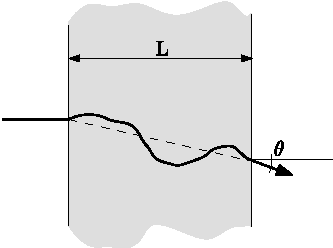
\includegraphics[width=0.78\columnwidth]{MultipleCoulombScat/MultipleScat.pdf}
    \caption{Left: Schematic representation of multiple coulomb scattering. Right: Schematic representation of electron backscattering.}
    \label{fig:PartScattering}
\end{figure}

It is very difficult to study any theory of multiple scattering for incident light particles such as electrons, due to the large number of scattering processes, not only by the atomic nuclei but also by the other electrons in the medium \parencite*[][]{ref:MultipleElec1}. Equation \ref{eq:multscat} is no longer valid in the case of a light particle \parencite*[][]{ref:MultipleElec2}, where large scattering angles are not rare. If an incident particle is scattered back of the material, it is called a backscattered particle. See figure \ref{fig:PartScattering} (right) for a schematic representation of the phenomenon.  Experimental information about this phenomenon has been intensively collected and from an empirical point of view, this phenomenon is well understood. However, attempts at a theoretical interpretation of the data have only limited success \parencite[][]{ref:BackScatTheo}.

For this document, we will only concern ourselves with the back-scattering electron yield ($BS_{el}$), which can be defined as the ratio between the number of outgoing primary electrons and the incident electron flux. Back-scattering of heavier particles, such as protons, is also possible. However, for our range of energies and materials, we consider this to be negligible.

\subsection{Path Length and Range}
\label{sec:Range}
The distance traveled by a particle inside a target until it loses all its energy can be quantified using the range. The range is an experimental concept, for which there are several definitions, all roughly relating to the same quantity \parencite*[][]{ref:Knoll}. In this document, the range (R) is defined as the penetration depth in a medium that reduces the number of incident particles to one-half. The maximum penetration depth ($R_{max}$) is defined as the depth in the absorbing medium beyond which no particles are observed to penetrate. Finally, the total path length describes the distance traveled by the particle measured along the actual path of the particle. Figure \ref{fig:RangeVsPathLength} illustrates the differences between these definitions. 

\begin{figure}[h]
    \centering
    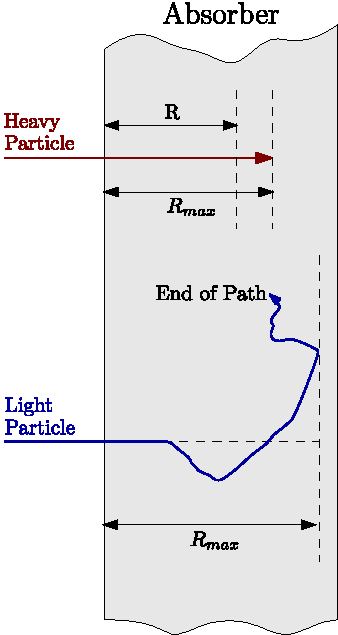
\includegraphics[width=0.9\columnwidth]{RangeVsPath/RangeVsPath.pdf}
    \caption{Schematic diagram of charged particle penetration into absorbing medium. Left: Heavy charged particle. Right: Light Charged particle.}
    \label{fig:RangeVsPathLength}
\end{figure}

The range highly depends on the type of particle, its energy and on the material through which it passes through. For a heavy particle that losses energy through ionization and atomic excitation, the range (R) can be calculated through the Continuous Slowing Down Approximation (CSDA): 

\begin{equation}
    R_{CSDA} = \int_{0}^{E_0} \left( \frac{dE}{dx} \right)^{-1} dE
    \label{eq:rangeCSDA}
\end{equation}

Where $E_0$ is the initial particle energy. This approximation assumes a smooth path, without hard collisions and large scattering angles. Some examples of analytical derivations of this equation can be found in \parencite*[][]{ref:CSDA}. The CSDA range for heavy non-relativistic charged particles, of mass $M_0$ and energy $E_k$, in a given absorber can be written in terms of the proton CSDA range ($R^{p}_{CSDA}$)as follows: 

\begin{equation}
    R_{CSDA}^{M_0} \left( E_K \right)= \frac{1}{Z^2} \left(\frac{M_0}{m_p}\right) R_{CSDA}^{p}\left[ E_K \frac{m_p}{M_0}\right]
\end{equation}

Where $M_p$ is the proton mass and Z is the atomic number of the incident ion. This can be very useful, as the range of protons in a variety of absorbers has been extensively measured. For heavy charged particles, $R_{max} \sim R_{CSDA}$ in all types of absorbing media. 

In the case of light particles, this CSDA approximation is not valid due to the very tortuous path that they experience in the absorbing medium. In this case, the CSDA range can be up to twice the average path for high Z absorbers ($R_{max} = 1/2 R_{CSDA}$). A useful quantity in the case of light particles is called the radiation length ($X_0$), usually measured in $g cm^2$. This gives us a mean distance over which high-energy particle losses all but $1/e$ of its energy by Bremsstrahlung. Different values for this quantity are available in literature, estimated with varying degrees of approximations. Some of these expressions can be found in \parencite*[][]{ref:radiationLength} and an example of an expression for high energetic electrons in high Z materials: 
\begin{equation}
    X_0 = \frac{716.405 A}{Z\left(Z+1\right)ln\left(183 Z^{-1/3}\right)}
    \label{eq:radiationlength.}
\end{equation}

\subsection{Types of Absorbers}

We will distinguish between thin and thick absorbers. In thin absorbers, only a few collisions of the projectile with the target atoms are likely to happen. Contrarily, in thick absorbers, a projectile experiences many collisions and the projectile energy lost by the incident particle is considerable. One can consider a target to be thin when the range of the incident particles is much larger than the thickness of the material ($R(E_k) >> L$). For thin absorbers, the energy loss is small and the stopping power doesn't change much along the length of the material. The total energy loss in the absorber can be calculated as: 

\begin{equation}
    \Delta E = - \left(\frac{dE}{dx}\right)_{avg} \cdot L
    \label{eq:thinabs}
\end{equation}

Here, the trajectory of the particle is also assumed to be perfectly linear in the absorber. If the range of the particles in the material is comparable to the thickness or smaller, this approximation is no longer valid, as one would underestimate the real energy deposition in the material. The energy is lost, the probability of interactions with the absorber material increases, since the ionization interaction cross-sections are bigger for smaller energies. A plot representing the specific energy loss along the incident particle track is called the Bragg curve. Figure \ref{fig:Bragg} shows an example of Bragg curve in the case of 3 \si[]{\mega\electronvolt} protons in graphite. 

\begin{figure}[h]
    \centering
    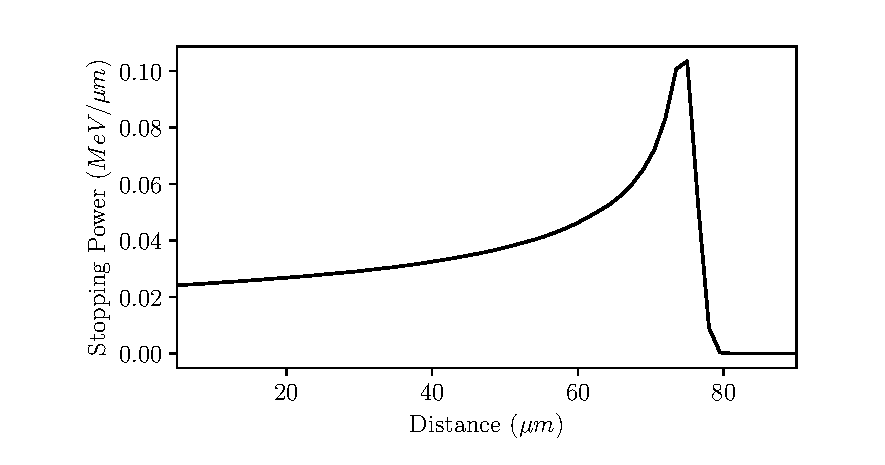
\includegraphics[width=1.0\columnwidth]{Bragg_Graphite/Bragg.pdf}
    \caption{Bragg peak of 3 \si[]{\mega \electronvolt} protons in Graphite. }
    \label{fig:Bragg}
\end{figure}

\section{Secondary Electron Theory}
\label{sec:SEY}
When a particle passes through the interface of a material, it will transfer energy to the electrons in the medium. Depending on the energy these electrons get, they can be excited to a higher energy level, or gain enough energy to be emitted from the material, this emission
process is known as Secondary Electron Emission (SEE) \parencite*[][]{ref:see1}. The SEE process can be generally divided into three consecutive steps:

\begin{enumerate}
    \item Generation Process: The energy required to ionize the atoms in the material is the minimum energy needed to create a secondary electron (SE). If the incident projectile is an ion containing electrons, these electrons can also be stripped off and produce further ionization. However, if the electrons from the incident ions are scattered off the material, they cannot be counted as secondary electrons. 
    \item Diffusion Process: While the SE travel through the material, they lose energy. This energy loss permits only a very shallow penetration depth of the low-energy electrons. For that reason, SE tends to be a surface phenomenon. 
    \item Emission Process: To be emitted from the surface, the SEs have to overcome the surface barrier potential \parencite*[][]{ref:see2}. The escape process is of particular importance because it determines the final shape of the secondary electron distribution. Moreover, the velocity vector, when reaching the surface, must allow the SE to escape. In the case of metals and semiconductors, a cosine-type angular distribution of SE is observed \parencite[][]{ref:angleSemi}
\end{enumerate}

\begin{figure}[h]
    \centering
    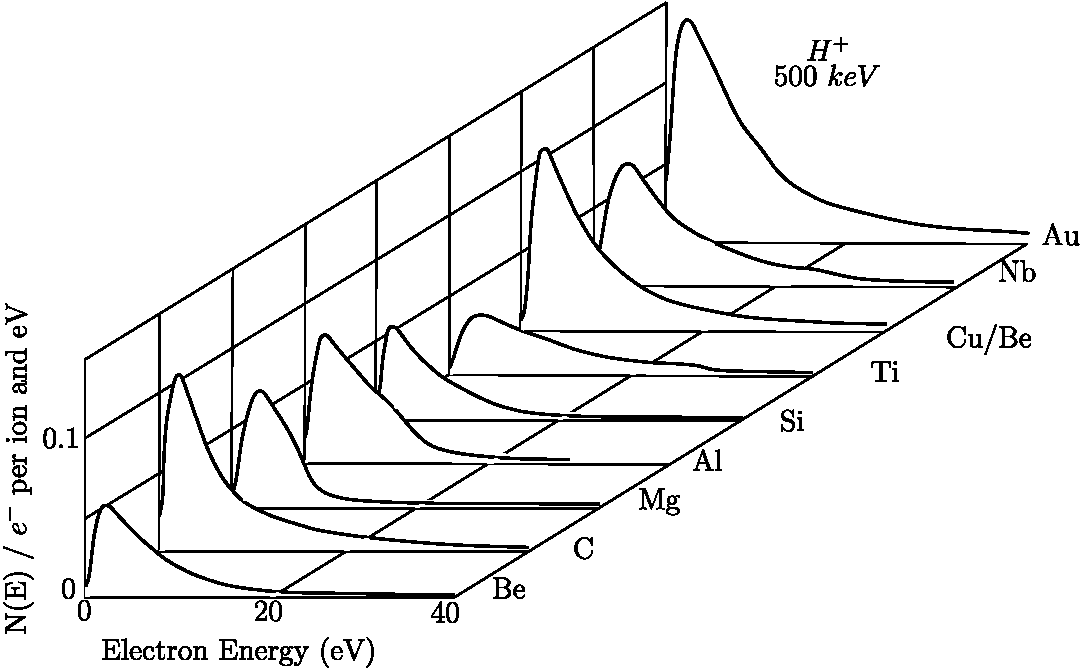
\includegraphics[width=0.9\columnwidth]{SEE_Spectra/SeeSpectra.pdf}
    \caption{Ion induced secondary electron spectra for a variety of metals. Incident ion: Proton 500 \si[]{\kilo \electronvolt}. From \parencite*[][]{ref:SEEspectra} }
    \label{fig:MetalsSE}
\end{figure}

Many experimental measurements of secondary electrons have been done since the discovery of this phenomenon in 1902, revealing some commonalities: In the case of SEE from metal surfaces \parencite*[][]{ref:see3},  The energy spectra of SE peak at about 1-5 eV; The full width of the peak is around 3-15 \si[]{\electronvolt}; It is commonly said that SE, in general, have an energy $< 50$ \si[]{\electronvolt}. Figure \ref{fig:MetalsSE} shows the spectra of SE emitted from different metals for an incident 500 \si[]{\kilo\electronvolt} proton. 

The main parameter describing the SEE is the Secondary Emission Yield (SEY). It describes the average number of electrons emitted per incident projectile. A semi-empirical treatment of SEY was formulated by E.J. Sternglass in 1957 \parencite*[][]{ref:SEY}. In this formulation, two sources of SE are considered. Firstly, the SE generated by small energy transfers from the incident particles to the target electrons. This first mechanism is the main contributor to the SEY. Secondly, a smaller contribution comes from the SE generated by delta electrons (defined in the following section). This formulation allows for the following numerical relation: 

\begin{equation}
    SEY = 0.01 L_S \left. \frac{dE}{dx}\right|_{el} \left[ 1+\frac{1}{1+5.4\cdot 10^{-6} E/A_p}\right]
    \label{eq:sey}
\end{equation}
\begin{equation}
    L_S = \left( 3.68\cdot 10^{-17} N_v Z^{1/3} \right)^{-1}
    \label{eq:LS}
\end{equation}

Here, E and $A_p$ are the kinetic energy and the mass of the projectile. $L_{s}$ is the characteristic length, which is of the order of the distance between inelastic collisions, and it is expressed in (\si[]{\centi\metre}). $N_v$ is the number of atoms per unit volume. $dE/dx$ is the energy deposition in the material due to interactions with the electrons. It should be expressed in eV/cm. As we saw previously (subsection\ref{sec:Bethe}), this term is greatly affected by the speed of the incident particle and its nature. 

The Secondary Emission Yield also depends on the angle of incidence of the incident particle. In the theory of Sternglass, the angular dependence is treated as a change in the effective penetration distance $L_{s}$. If the particle impacts at an angle different to the normal, the effective track length of the projectile extends by a factor $1/cos(\theta)$. In that case the corresponding SEY would be: 

\begin{equation}
    \frac{SEY(\theta)}{SEY(0)} = \frac{1}{cos(\theta)}
\end{equation}

Experimental values confirm this approximation for incident angles up to $70\deg$. However, if the incident particles are electrons, recent measurements show a different angular dependence \parencite*[][]{ref:seyAngleEl}: 
\begin{equation}
    \frac{SEY(\theta)}{SEY(0)} = e^{0.5 \left(1-cos(\theta)\right)}
\end{equation}

Early investigations of SEE already show a dependence of SEE on temperature \parencite*[][]{ref:SeyVsTemp}. Temperature seems to affect the escape probability. An increase in temperature results in increased vibrations of the atoms about their equilibrium position, which should reduce $L_{s}$, therefore increasing the Yield. Sternglass gives a rough quantitative hypothesis that goes as follows: 
\begin{equation}
    \frac{L_S (T_1)}{L_S(T_2)} = \frac{1+2.5\cdot 10^{-3}T_1}{1+2.5\cdot 10^{-3}T_2}
\end{equation}

Where $L_{S}(T_{1})$ is the characteristic length at $T_{1}$ and $L_{1}(T_{2})$ is the length at $T_{2}$. It is important to note that the semiempirical theory of secondary emission is only considered to be accurate for backward emission (projectile entering the target). As a first approximation, here we will consider that this formulation is also valid for rear-face emission. 

\subsection{Delta Rays}

Most frequently, the electrons generated by SE have low energy. However, if the energy transferred to the electron is above a few hundred \si[]{\electronvolt} (up to $T_{max}$), they might be able to generate further ionization on their own. An analytical formulation for the total number of $\delta$-rays produced from charged particle interactions was presented by Rossi in 1952 \parencite*[][]{ref:delta1}, and gives the distribution of $\delta$ rays for incident particles with energy $I \ll T \ll T_{max}$ as follows: 
\begin{equation}
    \frac{d^2N_{\delta}}{dTdx} = \frac{1}{2}Kz^2\frac{Z}{A}\frac{1}{\beta^2}\frac{F(T)}{T^2}
    \label{eq:deltaN}
\end{equation}

Where $T_{max}$ is given by equation \ref{eq:tmax}. The factor F is spin-dependent, but it is about unity for $ T \ll  T_{max}$. To calculate the total number of generated delta rays per unit of distance, one can integrate the previous equation from an arbitrary lower limit to the maximum energy for delta rays can get ($T_{max}$), described by Eq. \ref{eq:tmax}. 

